\section{Diseño del Sistema Redundante}

Aunque las arquitecturas redundantes suenan conceptualmente simples, su implementación real exige compromisos dolorosos entre robustez, costo y operatividad. Resulta revelador observar cómo las mejores soluciones surgen no de maximizar redundancia, sino de colocarla exactamente donde más duele.

\subsection{Arquitectura 1+1 y diversidad}

Uno de los desafíos persistentes al proponer diseños para VENESAT-2 radica en seleccionar el nivel adecuado de protección sin inflar innecesariamente la complejidad del sistema. La arquitectura base adoptada combina redundancia 1+1 en caliente a nivel de satélite y transpondedor con diversidad satelital y terrestre.

Esta configuración permite que un satélite de respaldo asuma carga de forma inmediata ante degradación o fallo del primario. Estudios sobre estaciones centrales redundantes han demostrado que este enfoque eleva significativamente la fiabilidad del enlace completo \cite{RedundantStation2015}. Se incorpora además diversidad de frecuencia (Ku/Ka) y de sitio para mitigar atenuación por lluvia.

La propuesta contempla dos satélites en posiciones orbitales cercanas (colocación) o el uso de capacidad contratada en un segundo operador GEO como respaldo temporal. Esta flexibilidad resulta clave en la fase de transición desde VENESAT-1.

\begin{figure}[h]
\centering
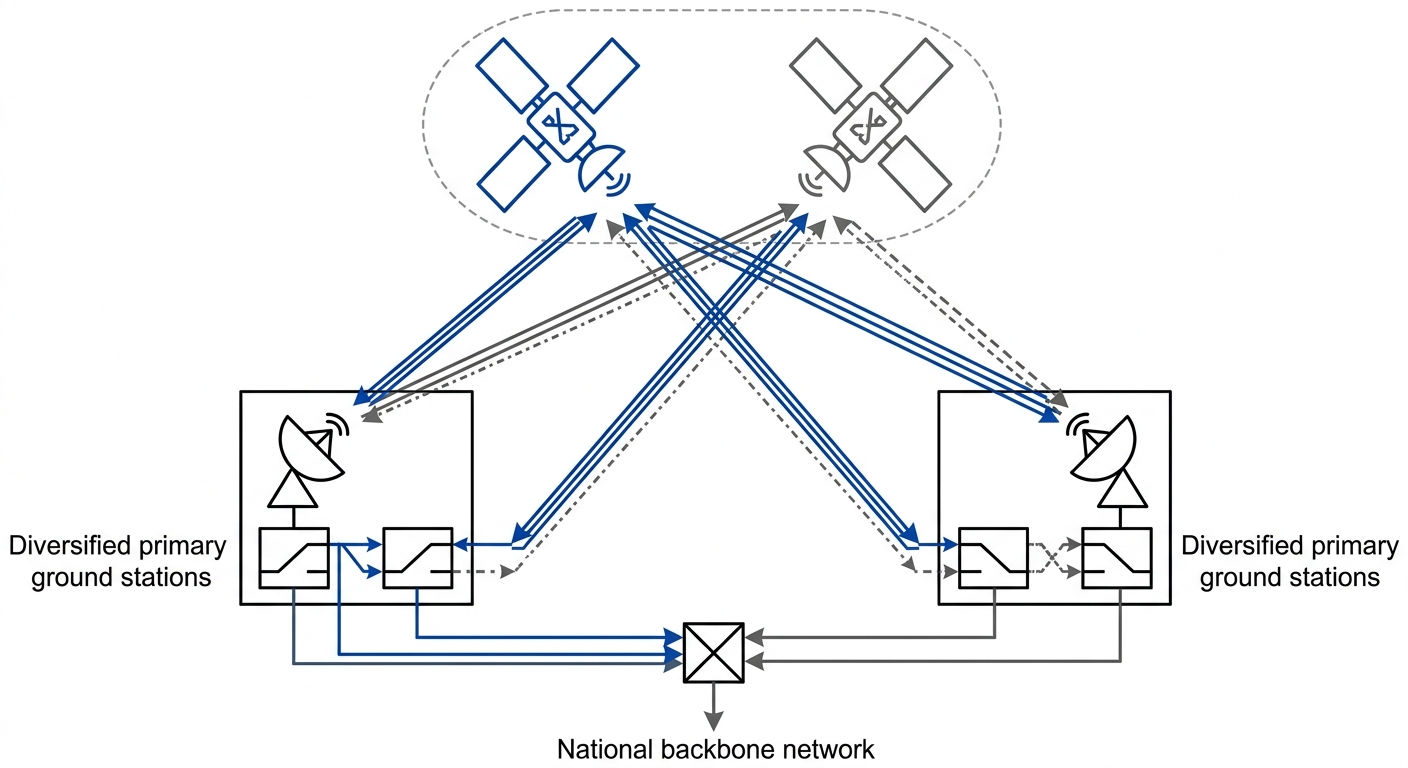
\includegraphics[width=\linewidth]{fig4.png}
\caption{Esquema de redundancia propuesto para el sistema de enlace satelital VENESAT-2}
\label{fig:esquema_redundancia}
\end{figure}

La Figura 3 ilustra el esquema general, donde se distinguen claramente las rutas primaria y redundante tanto en el segmento espacial como en el terrestre.

\subsection{Configuración de estaciones terrenas}

Lejos de ser meros repetidores, las estaciones terrenas constituyen el elemento crítico donde la redundancia genera mayor impacto operativo. Se propone un esquema de al menos dos estaciones principales geográficamente diversificadas: una en la región central-norte y otra en el sur-oriente, con regímenes pluviométricos diferentes.

Cada estación contará con antenas de 5.5 a 7.2 metros equipadas con sistemas de seguimiento automático y feeds duales Ku/Ka. La multi-conectividad satelital permite que las estaciones mantengan enlaces simultáneos con múltiples activos en órbita, mejorando notablemente la resiliencia ante fallos individuales \cite{MultiSatConnectivity2023}.

Esta disposición no solo mitiga efectos locales de lluvia intensa, sino que facilita mantenimiento sin interrupción total del servicio. En la práctica, una estación puede operar en modo primario mientras la otra permanece en hot-standby o soporta tráfico de baja prioridad.

\begin{table}[h]
\centering
\caption{Comparativa de costos relativos de alternativas de redundancia}
\label{tab:costos}
\begin{tabular}{lccc}
\hline
\textbf{Alternativa} & \textbf{Costo relativo} & \textbf{Disponibilidad} & \textbf{Complejidad operativa} \\
\hline
1+1 Satelital simple & 1.0 & 99.8\% & Media \\
Diversidad de sitio & 1.4 & 99.92\% & Alta \\
Multi-satélite híbrida & 2.1 & >99.97\% & Muy alta \\
Híbrida + terrestre & 2.8 & >99.99\% & Alta \\
\hline
\end{tabular}
\end{table}

La Tabla 5 presenta una evaluación comparativa preliminar. Aunque la opción híbrida completa ofrece el mejor desempeño, su costo sugiere priorizar una implementación por fases.

\subsection{Protocolos de conmutación}

Particularmente llamativo es el hecho de que muchos sistemas fallan no por falta de redundancia, sino por la ineficiencia de los mecanismos que deciden cuándo y cómo activarla. Se diseñaron protocolos de conmutación basados en umbrales combinados de C/N, BER y estado de telemetría.

La conmutación automática debe ocurrir en menos de 3 segundos para servicios críticos, con opción de intervención manual desde el centro de control. Se implementan algoritmos de decisión que consideran tanto métricas instantáneas como tendencias a corto plazo (predicción de atenuación basada en radar meteorológico).

No obstante, cabe matizar que protocolos demasiado agresivos pueden generar oscilaciones innecesarias (flapping), mientras que umbrales conservadores reducen la efectividad de la redundancia. El diseño final incorpora modos de operación degradada y procedimientos de reversión automática una vez restauradas las condiciones nominales.

Este conjunto de decisiones de diseño busca equilibrar la experiencia internacional disponible con las realidades logísticas y presupuestarias venezolanas. Las secciones siguientes validarán si esta arquitectura propuesta cumple con los requisitos de factibilidad establecidos previamente.